%!TEX program = xelatex
%!TEX spellcheck = en_GB
\documentclass[final]{article}
% Include all project wide packages here.
%\usepackage{fullpage}
\usepackage[a4paper,margin=2.5cm,top=2cm]{geometry}
\usepackage{polyglossia}
\setmainlanguage{english}
\usepackage{csquotes}
\usepackage{graphicx}
\usepackage{pdfpages}
\usepackage{caption}
\usepackage[list=true]{subcaption}
\usepackage{float}
\usepackage{standalone}
\usepackage{import}
\usepackage{tocloft}
\usepackage{wrapfig}
\usepackage{authblk}
\usepackage{array}
\usepackage{booktabs}
\usepackage[title,titletoc]{appendix}
\usepackage{fontspec}
\usepackage{pgfplots}
\usepackage{tikz}
\usepackage[binary-units=true,quotient-mode=fraction]{siunitx}
\usepackage{units}
\usepackage{amsmath}
\usepackage{mathtools}
\usepackage{unicode-math}
\usepackage{rotating}
\usepackage[compact]{titlesec}
\usepackage{titletoc}
\usepackage{blindtext}
\usepackage{color}
\usepackage{enumitem}
\usepackage{tabularx}
\usepackage{titling}
\usepackage[final]{microtype}
\usepackage[%
siunitx,
fulldiodes,
europeanvoltages,
europeancurrents,
europeanresistors,
americaninductors,
smartlabels]{circuitikz}

\newcommand{\matlab}{{\textsc{matlab }}}

\usetikzlibrary{calc}
\usetikzlibrary{positioning}
\usetikzlibrary{automata}
\usetikzlibrary{arrows.meta}

\tikzstyle{every state}=[fill=tu-cyan,align=center,draw=black,line width=1pt,node distance=3cm,minimum width = 1.8cm]%for FSMs casper
\tikzstyle{every initial by arrow}=[initial text={Reset}]
\newcommand{\setpathasarrows}{\tikzstyle{every path}=[auto,line width=1.5pt,line cap=round,line join=round]}

\pgfplotsset{compat=newest}
\pgfplotsset{plot coordinates/math parser=false}
\usetikzlibrary{plotmarks}
\usepgfplotslibrary{patchplots}
\newlength\figureheight
\newlength\figurewidth
\newlength\bytewidth
\newlength\byteheight
\setlength\bytewidth{1cm}
\setlength\byteheight{6ex}

\tikzset{every axis/.style={xticklabel style={align=right}}}

\tikzstyle{byte}=[draw, fill=blue!20, minimum width=6cm,line width=0.4pt,node distance=-0.4pt, minimum height=\byteheight,text width=6cm,font={\fontsize{9pt}{0}\selectfont}]
\tikzstyle{data}=[byte, fill=red!20]
\tikzstyle{padding}=[byte, fill=green!20]
\tikzstyle{byte_small}=[draw, fill=blue!20, minimum width=1.5cm,line width=0.4pt,node distance=-0.4pt, minimum height=\byteheight,text width=1.5cm]
\tikzstyle{data_small}=[byte_small, fill=red!20]

\usepackage[
%backend=bibtex,
backend=biber,
	texencoding=utf8,
bibencoding=utf8,
style=numeric,
citestyle=numeric,
    sortlocale=en_US,
    language=auto,
    backref=true,
    abbreviate=false,
    seconds=true,
    date=edtf
]{biblatex}


\usepackage{listings}
\newcommand{\includecode}[4][c]{\lstinputlisting[caption=#2, escapechar=, style=#1,label=#4]{#3}}
\newcommand{\superscript}[1]{\ensuremath{^{\textrm{#1}}}}
\newcommand{\subscript}[1]{\ensuremath{_{\textrm{#1}}}}


\newcommand{\chapternumber}{\thechapter}
\renewcommand{\appendixname}{Appendix}
\renewcommand{\appendixtocname}{Appendices}
\renewcommand{\appendixpagename}{Appendices}


\setlist[enumerate]{labelsep=*, leftmargin=1.5pc}
\setlist[enumerate,1]{label=\arabic*., ref=\arabic*}
\setlist[enumerate,2]{label=\arabic*.,ref=\theenumi.\arabic*}
\setlist[enumerate,3]{label=\arabic*., ref=\theenumii.\arabic*}

%\setcounter{chapter}{-1} %start chapter numbers with 0

\usepackage{xr-hyper}
\usepackage[hidelinks]{hyperref} %<--------ALTIJD ALS LAATSTE
\usepackage[nameinlink,noabbrev,capitalise]{cleveref} %<------- Clever Ref moet na hyperref
\crefname{app}{Appendix}{Appendices}
%\renewcommand{\familydefault}{\sfdefault}


\setmainfont{Myriad Pro}[Ligatures={Common,TeX}]
%\setmathfont{Asana Math}
\setmathfont{Asana-Math.otf}
\setmonofont[Scale=0.9]{Lucida Console}
\newfontfamily\headingfont{Minion Pro}[Ligatures={Common,TeX}]


\sisetup{detect-all}

%Design colors
\definecolor{accent1}{RGB}{0,100,200}
\definecolor{accent2}{RGB}{0,50,100}
\definecolor{tu-cyan}{RGB}{0,166,214}

\newcommand{\hsp}{\hspace{20pt}}
% \titleformat{\chapter}[hang]{\Huge\headingfont}{\chapternumber\hsp\textcolor{accent2}{|}\hsp}{0pt}{\Huge\headingfont}

% \titleformat{name=\chapter,numberless}[hang]{\Huge\headingfont}{\hsp\textcolor{accent2}{|}\hsp}{0pt}{\Huge\headingfont}

% \titleformat{\section}[block]{\LARGE\headingfont}{\arabic{chapter}.\arabic{section}}{0.4em}{}
% \titleformat{\subsection}[block]{\Large\headingfont}{\arabic{chapter}.\arabic{section}.\arabic{subsection}}{0.4em}{}
% \titleformat{\subsubsection}[block]{\large\headingfont}{\arabic{chapter}.\arabic{section}.\arabic{subsection}.\arabic{subsubsection}}{0.4em}{}
\renewcommand{\arraystretch}{1.05}
\renewcommand{\baselinestretch}{1.1}
\titlespacing{\section}{0pt}{2ex}{1ex}
\titlespacing{\subsection}{0pt}{1ex}{0ex}
\titlespacing{\subsubsection}{0pt}{0.5ex}{0ex}

\renewcommand\cfttoctitlefont{\headingfont\Huge}
\renewcommand\cftloftitlefont{\headingfont\Huge}
\renewcommand\cftlottitlefont{\headingfont\Huge}
\setcounter{lofdepth}{2}
\setcounter{lotdepth}{2}


\setlength{\parindent}{0pt}
\setlength{\parskip}{0.5em}

\captionsetup{width=0.9\textwidth}

%SIuntix settings:
%default: 0V to 10V
%custom: 0 - 10V
\sisetup{range-phrase=--}
\sisetup{range-units=single}
\DeclareSIUnit\years{years}

%For code listings
\definecolor{black}{rgb}{0,0,0}
\definecolor{browntags}{rgb}{0.65,0.1,0.1}
\definecolor{bluestrings}{rgb}{0,0,1}
\definecolor{graycomments}{rgb}{0.4,0.4,0.4}
\definecolor{redkeywords}{rgb}{1,0,0}
\definecolor{bluekeywords}{rgb}{0.13,0.13,0.8}
\definecolor{greencomments}{rgb}{0,0.5,0}
\definecolor{redstrings}{rgb}{0.9,0,0}
\definecolor{purpleidentifiers}{rgb}{0.01,0,0.01}


\lstdefinestyle{csharp}{
language=[Sharp]C,
showspaces=false,
showtabs=false,
breaklines=true,
showstringspaces=false,
breakatwhitespace=true,
escapeinside={(*@}{@*)},
columns=fullflexible,
commentstyle=\color{greencomments},
keywordstyle=\color{bluekeywords}\bfseries,
stringstyle=\color{redstrings},
identifierstyle=\color{purpleidentifiers},
basicstyle=\ttfamily\small}

\lstdefinestyle{c}{
language=C,
showspaces=false,
showtabs=false,
breaklines=true,
showstringspaces=false,
breakatwhitespace=true,
escapeinside={(*@}{@*)},
columns=fullflexible,
commentstyle=\color{greencomments},
keywordstyle=\color{bluekeywords}\bfseries,
stringstyle=\color{redstrings},
identifierstyle=\color{purpleidentifiers},
}

\lstdefinestyle{matlab}{
language=Matlab,
showspaces=false,
showtabs=false,
breaklines=true,
showstringspaces=false,
breakatwhitespace=true,
escapeinside={(*@}{@*)},
columns=fullflexible,
commentstyle=\color{greencomments},
keywordstyle=\color{bluekeywords}\bfseries,
stringstyle=\color{redstrings},
identifierstyle=\color{purpleidentifiers}
}

\lstdefinestyle{vhdl}{
language=VHDL,
showspaces=false,
showtabs=false,
breaklines=true,
showstringspaces=false,
breakatwhitespace=true,
escapeinside={(*@}{@*)},
columns=fullflexible,
commentstyle=\color{greencomments},
keywordstyle=\color{bluekeywords}\bfseries,
stringstyle=\color{redstrings},
identifierstyle=\color{purpleidentifiers}
}

\lstdefinestyle{xaml}{
language=XML,
showspaces=false,
showtabs=false,
breaklines=true,
showstringspaces=false,
breakatwhitespace=true,
escapeinside={(*@}{@*)},
columns=fullflexible,
commentstyle=\color{greencomments},
keywordstyle=\color{redkeywords},
stringstyle=\color{bluestrings},
tagstyle=\color{browntags},
morestring=[b]",
  morecomment=[s]{<?}{?>},
  morekeywords={xmlns,version,typex:AsyncRecords,x:Arguments,x:Boolean,x:Byte,x:Char,x:Class,x:ClassAttributes,x:ClassModifier,x:Code,x:ConnectionId,x:Decimal,x:Double,x:FactoryMethod,x:FieldModifier,x:Int16,x:Int32,x:Int64,x:Key,x:Members,x:Name,x:Object,x:Property,x:Shared,x:Single,x:String,x:Subclass,x:SynchronousMode,x:TimeSpan,x:TypeArguments,x:Uid,x:Uri,x:XData,Grid.Column,Grid.ColumnSpan,Click,ClipToBounds,Content,DropDownOpened,FontSize,Foreground,Header,Height,HorizontalAlignment,HorizontalContentAlignment,IsCancel,IsDefault,IsEnabled,IsSelected,Margin,MinHeight,MinWidth,Padding,SnapsToDevicePixels,Target,TextWrapping,Title,VerticalAlignment,VerticalContentAlignment,Width,WindowStartupLocation,Binding,Mode,OneWay,xmlns:x}
}

\lstdefinestyle{python}{
language=Python,
showspaces=false,
showtabs=false,
breaklines=true,
showstringspaces=false,
breakatwhitespace=true,
escapeinside={(*@}{@*)},
columns=fullflexible,
commentstyle=\color{greencomments},
keywordstyle=\color{bluekeywords}\bfseries,
stringstyle=\color{redstrings},
identifierstyle=\color{purpleidentifiers},
}

%defaults
\lstset{
basicstyle=\ttfamily\scriptsize ,
extendedchars=false,
numbers=left,
numberstyle=\ttfamily\tiny,
stepnumber=1,
tabsize=4,
numbersep=5pt
}
\addbibresource{../../.library/bibliography.bib}
\begin{document}
\section{Implementation}
\label{sec:implementation}

All custom embedded systems side code was written in C++ in stead of C.
Note that existing code like drivers and the software SDK was not rewritten to C++, but rather included as \texttt{extern "C"} to ensure compatibility.

\subsection{Communication}
The communication protocol is based on \SI{20}{\byte} fixed-length packets.
This size was chosen to properly fit into Bluetooth Low Energy frames.
The packet layout is as shown in \cref{fig:packet-format}
Some examples are shown in \cref{fig:packet-examples}.
The provided receive and transmit queues were used for the implementation, with an altered depth of \SI{240}{\byte} to fit an integer amount of \SI{20}{\byte} packets.
The receive function scans the input with a constant moving window for the header bytes, and when found receives the packet and passes it to handle packet.
If the type of packet requires an acknowledgement, the \texttt{ackNumber} field is copied and an acknowledgement packet is sent.

\subsection{System}
\label{ssec:implementation-system}
The system is built using a continuous loop (\texttt{void busywork()}) that runs as fast as possible.
And a timer that set a flag at \SI{100}{\hertz}, this triggers the \texttt{void tick()} function.
A hardware interrupt triggers the retrieval of the DMP sensor values from the MPU, also at \SI{100}{\hertz}.
This results in a near perfect \SI{100}{\hertz} execution rate of the tick function with a maximum delay of one DMP retrieval latency, as shown in \cref{ssec:module-latency}.
All other interval function are implemented as a division of the main loops frequency, so telemetry runs at \SI{10}{\hertz}, and the blue LED runs at \SI{1}{\hertz}, with dividers of 10 en 100 respectively.

The main function that handles mode changes and checks if they are valid is \texttt{void set\_mode(FlightMode)} where \texttt{FlightMode} is the type of the flight mode parameter.
This function returns depending on the current mode the state of the inputs and/or calibration values whenever or not the mode switch is acceptable.
If it's not, an exception packet is sent.

\subsection{Control}
%TODO[E]: The functions control (and possibily control_fast)

\begin{equation}
out = target_{lift} - P_{height} \cdot (target_{pressure} - current_{pressure})
\label{eq:control-height}
\end{equation}
%target is de setpoint, current is hier dat dus de baro waarde

\begin{equation}
out = P_{yaw} \cdot (target_{yaw} - rate_{yaw})
\label{eq:control-yaw}
\end{equation}
%target is de setpoint (rate), rate is hier dat dus de gyro waarde

\begin{equation}
out = P_1 \cdot (target_{roll,pitch} - current_{roll,pitch}) - P_2 \cdot rate_{roll,pitch}
\label{eq:control-roll-pitch}
\end{equation}
%target is de setpoint, current is hier dat dus de DMP waarde
%rate is de gyro rate (sp,sq)


\subsection{Logging}
All important information is written on a per-event basis, so telemetry data is written when telemetry is sent, sensor data is written when it is retrieved and so on.
The packets are variable length and do not contain a checksum.
The first thing written is a time stamp and then the packet type, this makes sure that parsing the binary back will be possible and straightforward.
When the flash is full the logging automatically disengages, and because the function state is included in the telemetry packet to the PC the PC also knows this.
When the dumping mode is activated the transmit buffer is filler to half, and the packets are put in the buffer as quickly as the transmission allows.
This makes for a quick transmission of the full binary data.

\subsection{Dashboard}
The Dashboard application is written in C\# for ease and speed of development.
Creating a GUI and implementing the threads shown in \cref{ssec:architecture-dashboard} is decidedly easier and more straightforward using the .NET framework than it is using any native toolkit.

The smartphone control feature was implemented as a web application using the \texttt{DeviceOrientationEvent} JavaScript API that enables convenient access to the orientation in pitch, yaw and roll of a handheld device.
The application is served by a simple web server built into the dashboard application.

Joystick and keyboard input is acquired using DirectInput, which has a very nice API and has a very low input lag.
All input axes except the Lift axis are scaled using an exponential curve, this way the control input near the middle is more fine grained, giving better control and making small adjustments easier.
A little deadzone was added as well, and before any values will be sent all input values will have to pass through their deadzone to active the actual RC control commands.
This because DirectInput does only report changes in joystick position so the throttle lever might be in a non-zero position after starting the application and the first movement will create a throttle spike to the motors.

\begin{figure}[H]
    \begin{subfigure}[b]{0.6\textwidth}
    \centering
        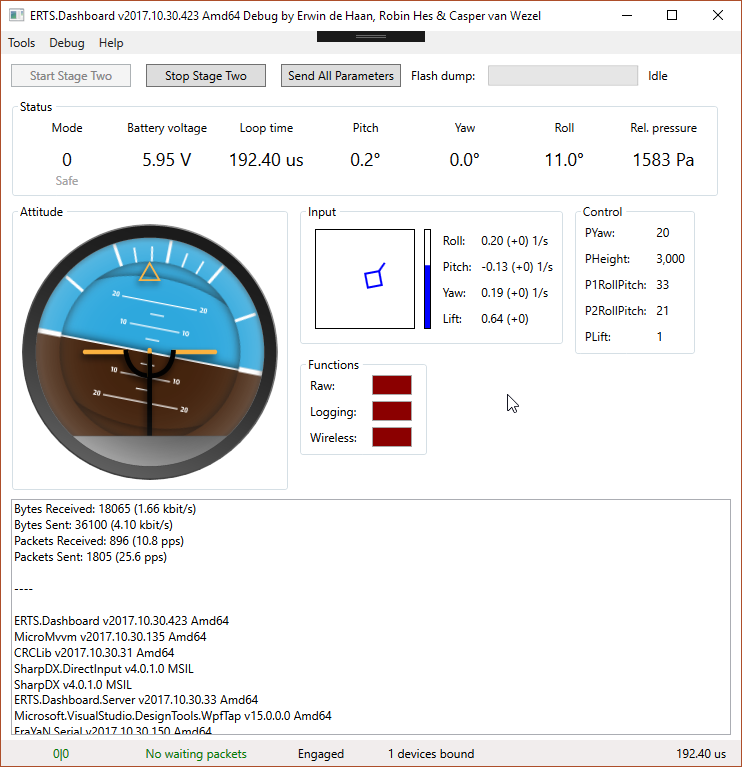
\includegraphics[height=10cm]{resources/dashboard-gui.png}
        \caption{The computer side dashboard UI.}
        \label{fig:pc-dashboard-gui}
    \end{subfigure}
    ~
    \begin{subfigure}[b]{0.4\textwidth}
    \centering
        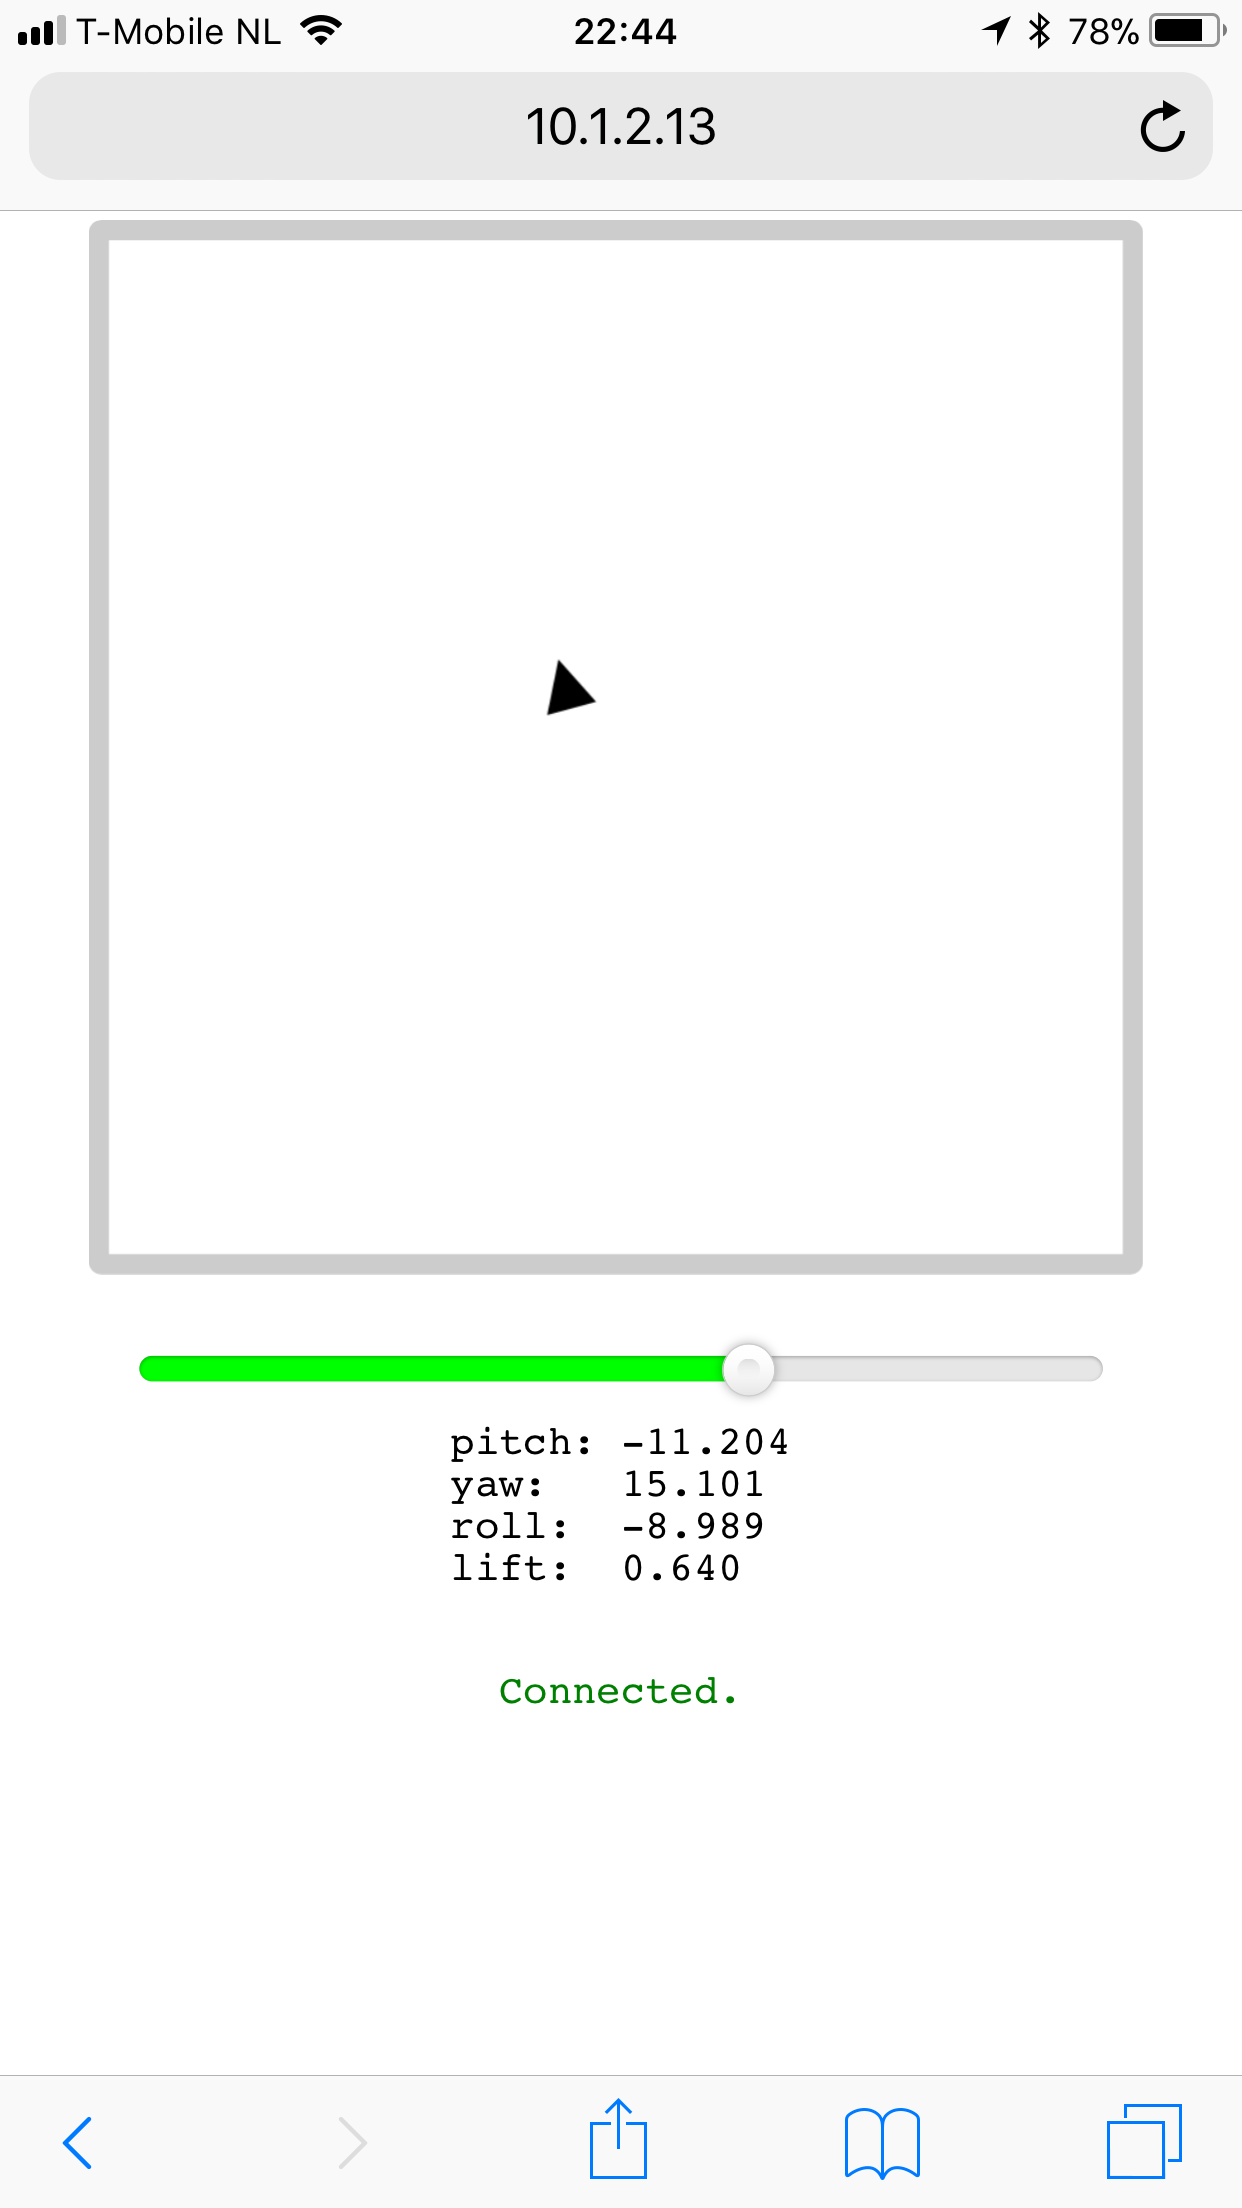
\includegraphics[height=10cm]{resources/phone-gui.PNG}
        \caption{The phone control UI.}
        \label{fig:phone-control-gui}
    \end{subfigure}
    \caption{The system UIs.}
    \label{fig:system-guis}
\end{figure}

\section{Division of work}
The authoring tags are written in the header files where possible as required.
Due to the limited nuance allowed in said tags, a quick overview is given in \cref{tab:work-division}.

\begin{table}[H]
    \caption{Coarse division of work during the project}
    \label{tab:work-division}
    \centering
    \begin{tabular}{lp{12cm}}
    \toprule
    Module                   & Notes \\
    \midrule
    ES-side architecture & Provided or tweaked/written by Robin \\
    ES-side control & Robin wrote most of the control code for manual, yaw, full and height control, with Casper taking the mixing of the motors. \\
    ES-side communication & Written in part by Erwin and Robin. Initial translation of C\# classes done by Robin.\\
    ES-side state handling & Initial design by Casper, written by Robin \\
    ES-side logging & Written by Casper \\
    ES-side Log dumping & Initial code by Casper, final finishing touches by Erwin \\
    Other ES-side code & Either provided or tweaked/written by Robin and tweaks by Erwin \\
    \midrule
    PC-side architecture & Written by Erwin \\
    PC-side control & Written by Erwin \\
    PC-side communication & Written by Erwin \\
    PC-side user interface & Written by Erwin, Initial binding design and ViewModel by Robin \\
    PC-side visualization & Written by Erwin \\
    PC-side log dumping & Written by Erwin \\
    PC-side http server & Written by Erwin \\
    Other PC-side modules & Written by Erwin, tweaks by Robin \\
    \midrule
    Phone-side input & Written by Robin, tweaks by Erwin \\
    SDL UI prototype & Written by Robin \\
    Protocol prototypes & Written by Erwin \\
    Flash binary parsing & Written by Erwin \\
    \bottomrule
    \end{tabular}
\end{table}
\end{document}